\usetikzlibrary{calc,positioning} % used to give coordinates
\usetikzlibrary{decorations.pathmorphing} % curved/coiled lines for photon and gluon
\usetikzlibrary{decorations.markings} % arrows, etc.
\usetikzlibrary{decorations.pathreplacing}
\usetikzlibrary{shapes}

  \pgfdeclaredecoration{single line}{initial}{ 
    \state{initial}[width=\pgfdecoratedpathlength-1sp]{\pgfpathmoveto{\pgfpointorigin}} 
    \state{final}{\pgfpathlineto{\pgfpointorigin}} 
  } 

\tikzset{
    % propagator styles
    susy_spin0/.style={dashed,line width=2pt,red},
    spin0/.style={dashed,line width=2pt},
    photon/.style={decorate,decoration={snake,amplitude=4pt,segment length=12pt,post length=0mm},line width=2pt},
    gluon/.style={decorate,decoration={coil,amplitude=5pt,segment length=8pt,aspect=1},line width=2pt},
    massvect/.style={decorate,decoration={snake},line width=2pt},
    fermion/.style={    line width=2pt,postaction={decorate, decoration={markings, mark=at position 0.55 with{\arrow{stealth}}} }},
    toextpot/.style={postaction={decorate,decoration={markings,mark=at position 1 with {\draw (-2pt,-2pt) -- (2pt,2pt);\draw (-2pt,2pt) -- (2pt,-2pt);}}}},
    arclabel/.style={preaction={decorate,decoration={markings,mark=at position .5 with {\node[void] at (0,0) [label=#1]{};}}}},
    %
    % These prevent the path from being drawn -> needs to be done twice
    momarrowr/.style={decorate,decoration={markings,mark=at position .5 with { \draw[->] (-2.5mm,-2.5mm) -- node [label=#1]{} (2.5mm,-2.5mm); }}},
    momarrowl/.style={decorate,decoration={markings,mark=at position .5 with { \draw[->] (-2.5mm,+2.5mm) -- node [label=#1]{} (2.5mm,2.5mm); }}},
    %
    % node styles (internal vertices, ``blobs'', external line starting points)
    vertex/.style={circle,draw,fill=black,inner sep=0pt,minimum size=.8mm},
    blob/.style={circle,draw=black!100,fill=black!35,inner sep=1pt,minimum size=5mm},
    oval/.style={ellipse,minimum height=13mm,minimum width=11mm,draw=black!100,fill=black!35,inner sep=1pt,line width=2pt},
    void/.style={inner sep=0pt,minimum size=0pt},
    counterterm/.style={lamp,draw,inner sep=0pt,minimum size=6pt},
    raiseline/.style={decorate, decoration={single line, raise=#1}, line width=2pt},
    rpv/.style={circle, draw=blue, fill=blue!35, inner sep=1pt, minimum size=3mm, line width=2pt}
}

\begin{center}
  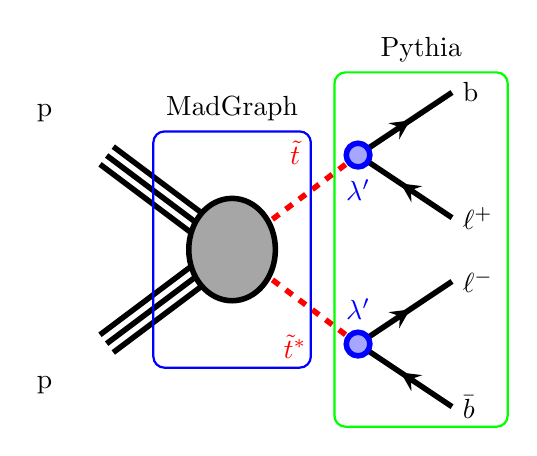
\begin{tikzpicture}[scale=0.8]
    \node[void] (in_1) at (-2,+1.5) {};
    \node[void] (in_2) at (-2,-1.5) {};

    \node[void] (emptyblob) at (0,0) {};

    \node[void] (v_u_int_1) at (2,+1.5) {};
    \node[void] (v_d_int_1) at (2,-1.5) {};

    \node[void] (out_u_1) at (3.5,+2.50) [label={[label distance=0pt]+0:{b}}]{} {};
    \node[void] (out_d_1) at (3.5,-2.50) [label={[label distance=0pt]+0:{$\bar{\text{b}}$}}]{} {};

    \node[void] (out_u_2) at (3.5,+0.50) [label={[label distance=0pt]+0:{$\ell^{+}$}}]{} {};
    \node[void] (out_d_2) at (3.5,-0.50) [label={[label distance=0pt]+0:{$\ell^{-}$}}]{} {};

    % Input proton 1
    \draw[raiseline=0]  (in_1) -- node [label={[label distance=40pt]+147:{p}}]{} (emptyblob);
    \draw[raiseline=4]  (in_1) -- (emptyblob);
    \draw[raiseline=-4] (in_1) -- (emptyblob);

    % Input proton 2
    \draw[raiseline=0]  (in_2) -- node [label={[label distance=40pt]-147:{p}}]{} (emptyblob);
    \draw[raiseline=4]  (in_2) -- (emptyblob);
    \draw[raiseline=-4] (in_2) -- (emptyblob);

    % stop decay
    \draw[susy_spin0] (emptyblob) -- node [label={[label distance=5pt]+90:{$\tilde{t}$}}]{} (v_u_int_1);
    \draw[fermion]    (v_u_int_1) -- (out_u_1);
    \draw[fermion]    (out_u_2) -- (v_u_int_1);

    % anti-stop decay
    \draw[susy_spin0] (emptyblob) -- node [label={[label distance=5pt]-90:{$\tilde{t}^{*}$}}]{} (v_d_int_1);
    \draw[fermion] (out_d_1) -- (v_d_int_1);
    \draw[fermion] (v_d_int_1) -- (out_d_2);

    \node[oval] (blob) at (0,0)  {};
    \node[rpv] (rpv) at (v_u_int_1) [label={[label distance=0pt,color=blue]-90:{$\lambda'$}}]{} {};
    \node[rpv] (rpv) at (v_d_int_1) [label={[label distance=0pt,color=blue]+90:{$\lambda'$}}]{} {};

    % \draw[blue,  thick, rounded corners] (-1.1, -1.7) (+1.3, +1.7);
    % \draw[green, thick, rounded corners] (+1.4, -3.0) (+4.2, +3.0);

    \node at (emptyblob) [draw, rectangle, rounded corners, minimum width=2cm,
                          minimum height=3cm, blue, thick, label=MadGraph] {};
    \node at (3,0)  [draw, rectangle, rounded corners, minimum width=2.2cm,
                     minimum height=4.5cm, green, thick, label=Pythia] {};

  \end{tikzpicture}
\end{center}
